\chapter{Discussion}\label{chap:discussion}


%Discuss the results. What is the outcome of your experimetns?

In this section, we will shortly discuss our results then extensively compare our work to the existing literature while trying to explain some of the differences. It will follow a section describing the limitations and possible extensions of our work. Finally, we will conclude this chapter with a section that describes the problems we encountered made during the implementation such that they can be avoided by others in the future.

\section{Our work}
In this section, we will quickly discuss our findings, and try to give some explanation to it.  
\subsection{Shuffling and learning rate with SGD}
As shown in figures \ref{fig:results_sgd}, \ref{fig:results_mom} and \ref{fig:results_nag}, the model, when using SGD as an optimizer,  was able to use a higher learning rate when the input was shuffled as when not. Therefore arises the questions why those this phenomena happen. One possibility is that the model is presented with a slightly different loss function every time, which is closer to the optimal loss function, therefore the steps taken by the optimizer are closer to the optimum and can, therefore, be bigger. Another explanation to why this did not happen to advanced optimizers is that we used a batched version of SGNS. Theretofore when not shuffled the optimizer often has the average value for some words, so that the gradient will be a rough estimation of the true gradient, and can, therefore, be imprecise. This is counter-attacked by advanced optimizers as they have adaptive learning rates.
\subsubsection{Large differences with NAG and SGD when using shuffling}
As shown in figures \ref{fig:results_sgd} and \ref{fig:results_nag}, plain SGD, and Nesterov Accelerated gradient, greatly differ in their convergence time when using shuffling into comparison when not. We attribute these results partially to a good random initialization guess and not only input shuffling. Due to a lack of time these results where not replicate more than once. 

\section{Related Work}
In this section, we will compare our work to related work. We will first compare us to the baseline model, the original C implementation from Mikolov et al \cite{Mikolov}. As they did not use the same datasets as we, this will hinder the quality of the comparison. We, therefore, compare ourself extensively to Gensim \cite{gensim}. Gensim is optimized to have a very high throughput which allowed us to, achieve a lot of computations. Furthermore, Gensim gave us access to the loss and the resulting word embeddings, which facilitated the comparison process. 

\subsection{word2vec}

As Mikolov et al. published the original paper which introduced the SGNS, it is, of course, relevant to compare ourselves to their work. The first important thing to take under account is that Mikolov et al. only trained their model on a very large google news dataset incorporating more than 3 billion words. This makes the comparison of our work more difficult. But we will make some assumptions, as they could be of value if true. 
In their original paper, Mikolov et al. reported results from computations that took 1 and 3 epochs. We accord these good results, which clearly outperformed our SGD model and Gensim, to the very large dataset and furthermore, as a matter of fact, their results are better with 3 than with 1 epoch. We do not have any information about the convergence time or criterion. Hence it would be interesting to use their dataset for comparison. \\
One thing we can compare is the quality of our word embeddings. Mikolov et al. did not report any results on their model with the text8 dataset, but they, therefore, published their code. Which was then used by Ji et al \cite{intel} and they tested the model on the text8 dataset. They reported a word similarity of 0.63 on the word similarity task. This is obviously outperformed by all our models. We did not find any explanation on why those results differ as much. \\
The final assumption is that an advanced optimizer could maybe outperform SGD in terms of quality on a large data set. This will be discussed in further work.
 


\subsection{Gensim}
The training with Gensim has a lot of possible parameters an extended list can be found in the appendix. This section we will only describe the parameters we changed from the default setting.  The description of each parameter will be done in the following way: \\
\texttt{name} (type) -- \textit{Description} -- Value\\
Parameters:
\begin{itemize}
   \item \texttt{sentences} (iterable of iterables) -- \textit{Dataset} -- text8 document splitted into sentences of 20 words 
  \item \texttt{size}(int) – \textit{Dimensionality of the word vectors } -- 100
\item \texttt{window} (int) --\textit {Maximum distance between the current and predicted word within a sentence }-- 5
  \item  \texttt{min\_count }(int) --\textit{ Ignores all words with total frequency lower than this }-- 5
 \item   \texttt{workers} (int) -- \textit{ Use these many worker threads to train the model (=faster training with multicore machines) }-- 4 
\item    \texttt{sg} ({0, 1}) --\textit{ Training algorithm: 1 for skip--gram}--1
  \item  \texttt{negative} (int) --\textit{Number of negative samples}-- 10 
\item   \texttt{ ns\_exponent} (float) --\textit{ Exponent in the unigram distribution, when choosing random samples, as shown in Equation \ref{eq:unigram} }-- 0.75
\item    \texttt{alpha} (float) --\textit{ The initial learning rate. }-- 0.025
 \item   \texttt{min\_alpha} (float) --\textit{ Learning rate will linearly drop to min\_alpha as training progresses. }--0.0001
 \item   \texttt{sample} (float) --\textit{ Treshold for subsampling as described in Equation \ref{eq:sampling}. } -- 1e--4
  \item  \texttt{iter} (int) --\textit{ Number of iterations (epochs) over the corpus. }-- 10 
 \
  \item  \texttt{compute\_loss} (bool) --\textit{If True, loss is stored at the end of each batch}-- True
 \item   \texttt{callbacks} (iterable of CallbackAny2Vec) --\textit{ Set of functions that will be executed at given training times, used in order to follow the loss and the progress of the model in word similarity }-- see Appendix
\end{itemize}

\subsubsection{Gensim vs. SGD}
%TODO analyze runtime if you have time
First, as stated earlier, we are not going to compare ourselves to Gensim in runtime. This does not make any sense as first of all our code is written in pytorch in comparison to Gensim which is implemented in cython\footnote{https://rare-technologies.com/word2vec-in-python-part-two-optimizing/}, which is 23x faster then plain Numpy, we use pytorch that optimizes Matrix multiplication so the difference shouldn't be that big, but still makes a difference. Secondly, we did not use any other runtime optimization technique, as our main goal was to improve the convergence time.\\
There are a few interesting contradictions to note between Gensim and our own implementation of the SGNS. First of all the convergence time was not the same. There are different possibilities for why this could be the case. First, our batched approach could hinder performance in term of convergence as our loss function is not exactly the same. When a word appears more than once in our batch, the gradient will be an average over the gradients of each pair alone, as it is done by Gensim. Another difference between our implementation is the fact that Gensim checks whether negative samples are not equal to the context word. And if that is the case selects a new random sample. Therefore the learning of the input and output context is optimized. Yet another possibility is the decay of the learning rate used by Gensim. In fact, decaying the learning rate has been proven in a lot of work to decrease the convergence time. Gensim linearly decreases the learning rate, as we did not use this technique, the decay of the learning rate could help explain the noted differences.
The first hypothesis may be confirmed by the fact that when combined with input shuffling SGD does perform closer to Gensim, going from 11 to 7 epochs to converge, as input shuffling reduces the number of co-occurrence of the same word in a batch. Know the question arises if the 3 epochs, that Gensim is better, can be explained by the selection of better negative samples and the learning rate decay?

\subsubsection{Gensim vs. Adam}
The Adam optimizer did outperform the Gensim application in performance (only slightly: 0.01 correlation coefficient better) and convergence time. Adam converged in 2 epochs while Gensim in 4. To be sure of our results we ran each computation 40 times. The results can be  seen in Figure \ref{fig:gensim_vs_adam}.

\begin{figure}[H]
    \centering
            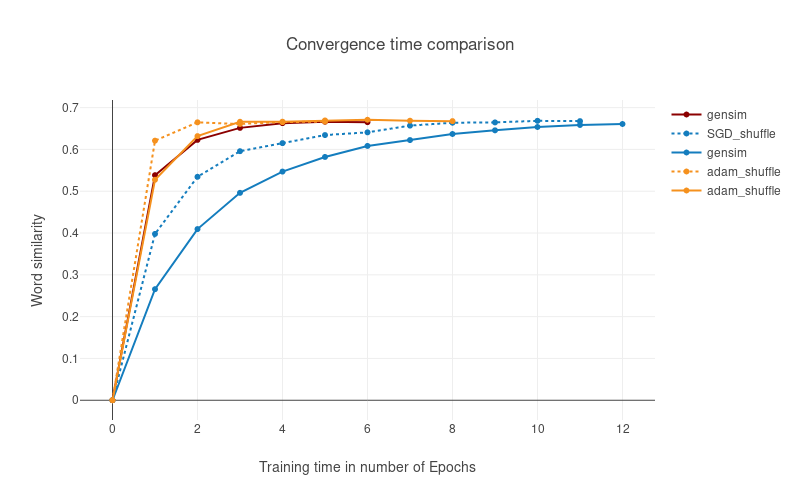
\includegraphics[scale=0.45]{images/gensim_vs_adam} 
    \caption{Training time Stochastic Gradient Descent with input Shuffling}
    \label{fig:gensim_vs_adam}
\end{figure}

\section{Challenges faced}
During our implementation we did encounter some problems, this section has the purpose of informing the scientific community to not make the same mistakes. 
\subsection{Using the wrong embeddings}
%TODO check projection vs input layer
To start with, we did not choose the same initialization value as Gensim in our word embeddings. We initialized the input layer with normal distribution between (-1,1), as opposed to Gensim which initializes all the weights to 0. We did this because as we first started, we did indeed do the same thing as Gensim, and initialized the projection layer with 0. But then our model did not seem to train well. Retrospectively we accord this to a learning rate that was too low. But back then we did not have the clarity of mind to see it, and instead changed the input layer initialization. After a few simulations, we saw that we did not perform as good as Gensim. And as we changed the initialization of the projection layer back to 0, as we already had adjusted the learning rate, we achieved good results. Therefore this is a recommendation to future work to not set the initialization to (-1,1).

\subsection{Batch size and loss function adjustements}\label{ssec:bs_lf}
During our experiments, we faced a moment where we needed to us a very high learning rate (50) to achieve good results. As this is the complete opposite of what is standard, we got suspicious. To remedy the problem we made a few changes. 
First, we needed to find a good batch size. During the above-explained raise of the learning rate, we used a batch size of 5000. We then decided to take a batch size of 2000.\\
 Secondly, at the same time, we did experiment with different loss functions. As our batched model does not have exactly the same loss function as introduced by Mikolov et al. \cite{mikolov}, we needed to find one that suited our goals the best. At the beginning of our experiment, we took the average of all the scores stored in our final matrix, as explained in \ref{ssec:b_SGM}. But then chose to take the sum as the training did not seem optimal.\\ 
 With these two changes, we did increase convergence time and word similarity, while at the same time having a usual learning rate. \\
 Know the question arises why this happened? Is this because of the shape of the loss function better suits our advanced optimizers? Or because the loss function is closer to its original form? Our hypothesis looks the following way: 
 When taking the average, our loss function is represented as follows:
 \begin{equation}
 \frac{-1}{b }* \sum_{x\in X} loss(x)
 \end{equation}
where $X$ is our batch and $b = |X|$. 
When taking the partial derivative of each parameter, the constant $ \frac{-1}{b }$ will remain the same. Therefore it's the same as taking the sum as the loss function and multiplying each gradient with $\frac{-1}{b }$. As our batch size was really high, i.e 2000 and 5000, this could highly influence the learning rate. This is also the conclusion of Goyal et al. \cite{fb}, that worked with very high batch sizes, i.e 8000: "When the minibatch size is multiplied by k, multiply the learning rate by k". We, therefore, did a small experiment to confirm this assumption. The results can be found in Table test. This shows empirically that this could be the main reason for the high learning rate.

\section{Future Work}
This work showed that the convergence time of the SGNS could be improved with the use of input shuffling and advanced optimizers. As with every work, there still exists possible extensions. First and foremost an aspect of our implementation that can be prejudicial is that we only extensively tested our model with one small dataset. Both of these aspects can be seen as problematic. By using a very small dataset we do not use the model in the condition it is most needed for, as the dataset used in practice usually consists of more than 1 billion words. There is a small argument that can be made for machine translation as the use of small parallel corpus is not unusual in this field. But the main issue with using only one data set it that it has been shown that some optimizers perform better with specific shapes of loss functions.  To make a compelling argument it's, therefore, necessary to show that our Model with the use of Input shuffling and Adam as it's optimizer also outperform Gensim with other data sets. We did show that this seems to be the case as Adam outperformed Gensim on the enwik9 dataset as well. But first, this experiment needs to be replicated a high number of times, i.e at least 40, so that the claim can hold consistently, and confirmed with other datasets as well.
Furthermore, our implementation did not outperform Gensim in runtime, as this was not the goal of our work. Therefore one could improve an already existing, optimized version, with input shuffling and advanced optimizers and should achieve a better runtime than Gensim.
